\documentclass[12pt]{report}
\usepackage[utf8]{inputenc}
\usepackage[T1]{fontenc}
\usepackage{amsmath,amsfonts,amssymb,stmaryrd}
\usepackage[english]{babel}
\usepackage{ifthen}
\usepackage{pdfpages}

%=============Affichage=======================
\usepackage{fullpage}
\usepackage{mathtools}
\usepackage{lmodern}
\usepackage{xcolor}
\usepackage{tikz}

\setlength{\topmargin}{-1.5cm}
\setlength{\textheight}{25cm}
\setlength{\textwidth}{16cm}
\setlength{\oddsidemargin}{-1.5cm}
\setlength{\evensidemargin}{50cm}

\newcommand{\rd}[1]{\textcolor{red}{#1}}
\newcommand{\g}[1]{\textcolor{lime}{#1}}
\newcommand{\dg}[1]{\textcolor{green}{#1}}
\newcommand{\blue}[1]{\textcolor{blue}{#1}}
\newcommand{\cy}[1]{\textcolor{cyan}{#1}}
\newcommand{\blz}{$\blacklozenge$}
\newcommand{\ns}{\\\indent\indent\vspace{0.25cm}}
\newcommand{\df}{$\equiv$ }
\setcounter{secnumdepth}{5}% profondeur de la table des matières
\usepackage{titlesec}


\titleformat{\chapter}[frame]
{\Huge}
{\filright\rmfamily\bfseries\Huge\enspace\thechapter\enspace}
{18pt}
{\rmfamily\huge\bfseries\filcenter}
% rmfamily=roman, sffamily = sans serif ou ttfamily =type writer
\usepackage[many]{tcolorbox} % Creation de box collorable pour le texte non intégré
\newtcolorbox{mybox}{colback=white,
colframe=red,arc=0mm}

\renewcommand*{\overrightarrow}[1]{\vbox{\halign{##\cr
 \tiny\rightarrowfill\cr\noalign{\nointerlineskip\vskip1pt}
 $#1\mskip2mu$\cr}}}

\newcommand*{\Coordp}[4]{%
 \ensuremath{{#1}\,
   \left\lvert
     \begin{matrix}
       #2\\
       #3\\
       #4
     \end{matrix}
   \right.% Ne pas oublier le délimiteur invisible.
 }}
 \newcommand{\divp}[2]
	{
	  \frac{\partial #1}{\partial #2}
	}

\newcommand{\divt}[2]
	{
	  \frac{d #1}{d #2}
	}

\newcommand{\divpsnd}[2]
	{
	  \frac{\partial^2 #1}{\partial #2^2}
	}

\newcommand{\divts}[2]
	{
	  \frac{d^2 #1}{d #2^2}
	}

\newcommand{\rem}[1]
{
\cy{\underline{\blz Remarque: }#1}\vspace{0.5cm}
}

\newcommand{\props}[1]
{
\begin{mybox}
\textbf{\rd{\underline{\blz Propriétés:} #1}}
\vspace{0.5cm}
\newline
}

\newcommand{\thetap}{\dot{\theta}}

\newcommand{\rot}[1]
{
\overrightarrow{rot}(\overrightarrow{#1})
}

\newcommand{\grad}[1]
{
\overrightarrow{grad}(\overrightarrow{#1})
}

\newcommand{\lapl}[1]
{
\Delta(\overrightarrow{#1})
}

\newcommand{\divs}[1]
{
div(\overrightarrow{#1})
}

\newcommand{\prope}
{
\end{mybox}
}

\newcommand{\defis}[1]
{
\begin{mybox}
\textbf{\rd{\underline{\blz Définition:} #1}}
\vspace{0.5cm}
\newline
}
\newcommand{\defie}
{
\end{mybox}
}
\newcommand{\discu}[1]
{
\blue{\underline{\blz Discussion:} #1}
}

\newcommand{\vs}
{
\vspace{0.25cm}
}
%=============================================

%\usepackage[cm]{aeguill}

%=============Mathématiques=================

%--------------Raccourcis:------------------
\newcommand{\R}{\mathbb{R}}
\newcommand{\C}{\mathbb{C}}
\newcommand{\N}{\mathbb{N}}
\newcommand{\Q}{\mathbb{Q}}
\newcommand{\Z}{\mathbb{Z}}
\newcommand{\K}{\mathbb{K}}
\newcommand{\M}{\mathcal{M}}

\newcommand{\abs}[1]{\left\lvert#1\right\rvert}
\DeclarePairedDelimiter{\ceil}{\lceil}{\rceil}

%Format de fonctions:
\newcommand{\fct}[5]
	{
	  \begin{array}{ccccc}
		#1 & : & #2 & \to & #3 \\
	    && #4 & \mapsto & #5 \\
	  \end{array}
	}

%===================TESTS===================

\begin{document}
\chapter{TD1 Logique Classique Propositionnelle}

\section{Exercice 1:}

\begin{enumerate}
  \item $(a \to b) \vee c$ est une formule bien formée car $(a \to b)$ est bien une formule bien formée et l'en semble forme un $(A \vee B)$ qui est bien formé dont on peut omettre les parenthèse extérieur car elle n'induise aucune intéraction avec un terme de la formuke

  \item $((a \to b) \vee c) \leftrightarrow \neg c$ est un formule mal formée car même si le terme de gauche est bien formé entre parenthèse car correspond à la question 1), elle reste mal formé car il manque les parenthèses sur $\neg c$ ce qui rend  $\leftrightarrow \neg c$ mal formée

  \item $\neg((a \to b) \vee c) \leftrightarrow ( a \vee b)$ est une formule mal formée car il manque les parenthèses sur $\neg (a \to b) \vee c$
\end{enumerate}

\section{Exercice: 2}

\begin{enumerate}
  \item \begin{align*}
            ((p \wedge q) \leftrightarrow (\neg(p \wedge q))) &\equiv (p \wedge q) \leftrightarrow (\neg(p \wedge q))
        \end{align*}
  \item \begin{align*}
           (((p \vee q)\vee r)\to (((\neg p)\wedge q)\to (p \wedge r))) &\equiv
            (p \vee q \vee r) \to ( ( \neg p \wedge q)\to (p \wedge r) )
        \end{align*}
  \item \begin{align*}
              (p \vee ((p \leftrightarrow q) \wedge ((\neg q) \to r))) & \equiv
              p \vee ( (p \leftrightarrow q) \wedge (\neg q \to r))
        \end{align*}
\end{enumerate}

\newpage

\section{Exercice 3}
\begin{enumerate}
  \item $ p \to  \neg p $ \\
        connecteur principal : $\to$\\
        profondeur: $2$\\
        nombre de sous-formules: $3$   $| (p \to  \neg p) $, $p$, $\neg p$
  \begin{center}
% Racine en Haut, développement vers le bas
\begin{tikzpicture}[xscale=1,yscale=1]
% Styles (MODIFIABLES)
\tikzstyle{fleche}=[->,>=latex,thick]
\tikzstyle{noeud}=[fill=yellow,circle,draw]
\tikzstyle{feuille}=[fill=yellow,circle,draw]
% Dimensions (MODIFIABLES)
\def\DistanceInterNiveaux{1.5}
\def\DistanceInterFeuilles{2}
% Dimensions calculées (NON MODIFIABLES)
\def\NiveauA{(-0)*\DistanceInterNiveaux}
\def\NiveauB{(-1.5)*\DistanceInterNiveaux}
\def\NiveauC{(-2.5)*\DistanceInterNiveaux}
\def\InterFeuilles{(1)*\DistanceInterFeuilles}
% Noeuds (MODIFIABLES : Styles et Coefficients d'InterFeuilles)
\node[noeud] (R) at ({(0.5)*\InterFeuilles},{\NiveauA}) {$\to$};
\node[feuille] (Ra) at ({(0)*\InterFeuilles},{\NiveauB}) {$p$};
\node[noeud] (Rb) at ({(1)*\InterFeuilles},{\NiveauB}) {$\neg$};
\node[feuille] (Rba) at ({(1)*\InterFeuilles},{\NiveauC}) {$p$};
% Arcs (MODIFIABLES : Styles)
\draw[fleche] (R)--(Ra);
\draw[fleche] (R)--(Rb);
\draw[fleche] (Rb)--(Rba);
\end{tikzpicture}
\end{center}

\item $(p \vee q) \to (p \wedge q) $\\
connecteur principal : $\to$\\
profondeur: $2$\\
nombre de sous-formules: $5$   $| ((p \vee q) \to (p \wedge q)) $,$(p \vee q)$,$(p \wedge q)$, $p$, $q$
\begin{center}
% Racine en Haut, développement vers le bas
\begin{tikzpicture}[xscale=1,yscale=1]
% Styles (MODIFIABLES)
\tikzstyle{fleche}=[->,>=latex,thick]
\tikzstyle{noeud}=[fill=yellow,circle,draw]
\tikzstyle{feuille}=[fill=yellow,circle,draw]
% Dimensions (MODIFIABLES)
\def\DistanceInterNiveaux{1.5}
\def\DistanceInterFeuilles{2}
% Dimensions calculées (NON MODIFIABLES)
\def\NiveauA{(-0)*\DistanceInterNiveaux}
\def\NiveauB{(-1)*\DistanceInterNiveaux}
\def\NiveauC{(-2)*\DistanceInterNiveaux}
\def\InterFeuilles{(1)*\DistanceInterFeuilles}
% Noeuds (MODIFIABLES : Styles et Coefficients d'InterFeuilles)
\node[noeud] (R) at ({(1.5)*\InterFeuilles},{\NiveauA}) {$\to$};
\node[noeud] (Ra) at ({(0.5)*\InterFeuilles},{\NiveauB}) {$\vee$};
\node[feuille] (Raa) at ({(0)*\InterFeuilles},{\NiveauC}) {$p$};
\node[feuille] (Rab) at ({(1)*\InterFeuilles},{\NiveauC}) {$q$};
\node[noeud] (Rb) at ({(2.5)*\InterFeuilles},{\NiveauB}) {$\wedge$};
\node[feuille] (Rba) at ({(2)*\InterFeuilles},{\NiveauC}) {$p$};
\node[feuille] (Rbb) at ({(3)*\InterFeuilles},{\NiveauC}) {$q$};
% Arcs (MODIFIABLES : Styles)
\draw[fleche] (R)--(Ra);
\draw[fleche] (Ra)--(Raa);
\draw[fleche] (Ra)--(Rab);
\draw[fleche] (R)--(Rb);
\draw[fleche] (Rb)--(Rba);
\draw[fleche] (Rb)--(Rbb);
\end{tikzpicture}
\end{center}

\item $\neg (p \vee (q \wedge r)) \to (p \wedge q) $\\
connecteur principal : $\to$\\
profondeur: $4$\\
nombre de sous-formules: $8$   $| (\neg (p \vee (q \wedge r)) \to (p \wedge q)) $,$\neg (p \vee (q \wedge r))$,$p \vee (q \wedge r)$,$p$,$(q \wedge r)$,$q$,$(p \wedge q)$,$r$
%:-+-+-+- Engendré par : http://math.et.info.free.fr/TikZ/Arbre/
\begin{center}
% Racine en Haut, développement vers le bas
\begin{tikzpicture}[xscale=1,yscale=1]
% Styles (MODIFIABLES)
\tikzstyle{fleche}=[->,>=latex,thick]
\tikzstyle{noeud}=[fill=yellow,circle,draw]
\tikzstyle{feuille}=[fill=yellow,circle,draw]
% Dimensions (MODIFIABLES)
\def\DistanceInterNiveaux{1.5}
\def\DistanceInterFeuilles{2}
% Dimensions calculées (NON MODIFIABLES)
\def\NiveauA{(-0)*\DistanceInterNiveaux}
\def\NiveauB{(-1)*\DistanceInterNiveaux}
\def\NiveauC{(-2)*\DistanceInterNiveaux}
\def\NiveauD{(-3)*\DistanceInterNiveaux}
\def\NiveauE{(-4)*\DistanceInterNiveaux}
\def\InterFeuilles{(1)*\DistanceInterFeuilles}
% Noeuds (MODIFIABLES : Styles et Coefficients d'InterFeuilles)
\node[noeud] (R) at ({(2)*\InterFeuilles},{\NiveauA}) {$\to$};
\node[noeud] (Ra) at ({(1)*\InterFeuilles},{\NiveauB}) {$\neg$};
\node[noeud] (Raa) at ({(1)*\InterFeuilles},{\NiveauC}) {$\vee$};
\node[feuille] (Raaa) at ({(0)*\InterFeuilles},{\NiveauD}) {$p$};
\node[noeud] (Raab) at ({(1.5)*\InterFeuilles},{\NiveauD}) {$\wedge$};
\node[feuille] (Raaba) at ({(1)*\InterFeuilles},{\NiveauE}) {$p$};
\node[feuille] (Raabb) at ({(2)*\InterFeuilles},{\NiveauE}) {$q$};
\node[noeud] (Rb) at ({(3.5)*\InterFeuilles},{\NiveauB}) {$\wedge$};
\node[feuille] (Rba) at ({(3)*\InterFeuilles},{\NiveauC}) {$p$};
\node[feuille] (Rbb) at ({(4)*\InterFeuilles},{\NiveauC}) {$q$};
% Arcs (MODIFIABLES : Styles)
\draw[fleche] (R)--(Ra);
\draw[fleche] (Ra)--(Raa);
\draw[fleche] (Raa)--(Raaa);
\draw[fleche] (Raa)--(Raab);
\draw[fleche] (Raab)--(Raaba);
\draw[fleche] (Raab)--(Raabb);
\draw[fleche] (R)--(Rb);
\draw[fleche] (Rb)--(Rba);
\draw[fleche] (Rb)--(Rbb);
\end{tikzpicture}
\end{center}
%:-+-+-+-+- Fin

\item $\neg ((\neg p \vee q) \leftrightarrow (q \wedge r)) \to q $\\
connecteur principal : $\to$\\
profondeur: $5$\\
nombre de sous-formules: $9$   $|$ $\neg ((\neg p \vee q) \leftrightarrow (q \wedge r)) \to q $, $q$,$\neg ((\neg p \vee q) \leftrightarrow (q \wedge r))$,$(\neg p \vee q) \leftrightarrow (q \wedge r)$,$\neg p \vee q$,$q \wedge r$,$\neg p$,$p$,$r$

%:-+-+-+- Engendré par : http://math.et.info.free.fr/TikZ/Arbre/
\begin{center}
% Racine en Haut, développement vers le bas
\begin{tikzpicture}[xscale=1,yscale=1]
% Styles (MODIFIABLES)
\tikzstyle{fleche}=[->,>=latex,thick]
\tikzstyle{noeud}=[fill=yellow,circle,draw]
\tikzstyle{feuille}=[fill=yellow,circle,draw]
% Dimensions (MODIFIABLES)
\def\DistanceInterNiveaux{1.5}
\def\DistanceInterFeuilles{2}
% Dimensions calculées (NON MODIFIABLES)
\def\NiveauA{(-0)*\DistanceInterNiveaux}
\def\NiveauB{(-1)*\DistanceInterNiveaux}
\def\NiveauC{(-2)*\DistanceInterNiveaux}
\def\NiveauD{(-3)*\DistanceInterNiveaux}
\def\NiveauE{(-4)*\DistanceInterNiveaux}
\def\NiveauF{(-5)*\DistanceInterNiveaux}
\def\InterFeuilles{(1)*\DistanceInterFeuilles}
% Noeuds (MODIFIABLES : Styles et Coefficients d'InterFeuilles)
\node[noeud] (R) at ({(2)*\InterFeuilles},{\NiveauA}) {$\to $};
\node[noeud] (Ra) at ({(1.5)*\InterFeuilles},{\NiveauB}) {$\neg$};
\node[noeud] (Raa) at ({(1.5)*\InterFeuilles},{\NiveauC}) {$\leftrightarrow$};
\node[noeud] (Raaa) at ({(0.5)*\InterFeuilles},{\NiveauD}) {$\vee$};
\node[feuille] (Raaaa) at ({(0)*\InterFeuilles},{\NiveauE}) {$q$};
\node[noeud] (Raaab) at ({(1)*\InterFeuilles},{\NiveauE}) {$\neg$};
\node[feuille] (Raaaba) at ({(1)*\InterFeuilles},{\NiveauF}) {$p$};
\node[noeud] (Raab) at ({(2.5)*\InterFeuilles},{\NiveauD}) {$\wedge$};
\node[feuille] (Raaba) at ({(2)*\InterFeuilles},{\NiveauE}) {$q$};
\node[feuille] (Raabb) at ({(3)*\InterFeuilles},{\NiveauE}) {$r$};
\node[feuille] (Rb) at ({(4)*\InterFeuilles},{\NiveauB}) {$q$};
% Arcs (MODIFIABLES : Styles)
\draw[fleche] (R)--(Ra);
\draw[fleche] (Ra)--(Raa);
\draw[fleche] (Raa)--(Raaa);
\draw[fleche] (Raaa)--(Raaaa);
\draw[fleche] (Raaa)--(Raaab);
\draw[fleche] (Raaab)--(Raaaba);
\draw[fleche] (Raa)--(Raab);
\draw[fleche] (Raab)--(Raaba);
\draw[fleche] (Raab)--(Raabb);
\draw[fleche] (R)--(Rb);
\end{tikzpicture}
\end{center}
%:-+-+-+-+- Fin
\item $((p \wedge (\neg q \to \neg q)) \wedge (\neg q \vee r)) \to (r \to \neg p) $\\
connecteur principal : $\to$\\
profondeur: $5$\\
nombre de sous-formules: $11$   $|$ $((p \wedge (\neg q \to \neg q)) \wedge (\neg q \vee r)) \to (r \to \neg p) $, $(r \to \neg p)$, $r$ , $\neg p$, $p$, $(p \wedge (\neg q \to \neg q)) \wedge (\neg q \vee r)$, $(p \wedge (\neg q \to \neg q)$,$(\neg q \vee r)$,$\neg q$,$q$,$(\neg q \to \neg q)$

%:-+-+-+- Engendré par : http://math.et.info.free.fr/TikZ/Arbre/
\begin{center}
% Racine en Haut, développement vers le bas
\begin{tikzpicture}[xscale=1,yscale=1]
% Styles (MODIFIABLES)
\tikzstyle{fleche}=[->,>=latex,thick]
\tikzstyle{noeud}=[fill=yellow,circle,draw]
\tikzstyle{feuille}=[fill=yellow,circle,draw]
% Dimensions (MODIFIABLES)
\def\DistanceInterNiveaux{1.5}
\def\DistanceInterFeuilles{2}
% Dimensions calculées (NON MODIFIABLES)
\def\NiveauA{(-0)*\DistanceInterNiveaux}
\def\NiveauB{(-1)*\DistanceInterNiveaux}
\def\NiveauC{(-2)*\DistanceInterNiveaux}
\def\NiveauD{(-3)*\DistanceInterNiveaux}
\def\NiveauE{(-4)*\DistanceInterNiveaux}
\def\NiveauF{(-5)*\DistanceInterNiveaux}
\def\InterFeuilles{(1)*\DistanceInterFeuilles}
% Noeuds (MODIFIABLES : Styles et Coefficients d'InterFeuilles)
\node[noeud] (R) at ({(3)*\InterFeuilles},{\NiveauA}) {$\to $};
\node[noeud] (Ra) at ({(2)*\InterFeuilles},{\NiveauB}) {$\wedge$};
\node[noeud] (Raa) at ({(1)*\InterFeuilles},{\NiveauC}) {$\wedge$};
\node[feuille] (Raaa) at ({(0)*\InterFeuilles},{\NiveauD}) {$p$};
\node[noeud] (Raab) at ({(1.5)*\InterFeuilles},{\NiveauD}) {$\to$};
\node[noeud] (Raaba) at ({(1)*\InterFeuilles},{\NiveauE}) {$\neg$};
\node[feuille] (Raabaa) at ({(1)*\InterFeuilles},{\NiveauF}) {$q$};
\node[noeud] (Raabb) at ({(2)*\InterFeuilles},{\NiveauE}) {$\neg$};
\node[feuille] (Raabba) at ({(2)*\InterFeuilles},{\NiveauF}) {$q$};
\node[noeud] (Rab) at ({(3.5)*\InterFeuilles},{\NiveauC}) {$\vee$};
\node[noeud] (Raba) at ({(3)*\InterFeuilles},{\NiveauD}) {$\neg$};
\node[feuille] (Rabaa) at ({(3)*\InterFeuilles},{\NiveauE}) {$q$};
\node[feuille] (Rabb) at ({(4)*\InterFeuilles},{\NiveauD}) {$r$};
\node[noeud] (Rb) at ({(5.5)*\InterFeuilles},{\NiveauB}) {$\to$};
\node[feuille] (Rba) at ({(5)*\InterFeuilles},{\NiveauC}) {$r$};
\node[noeud] (Rbb) at ({(6)*\InterFeuilles},{\NiveauC}) {$\neg $};
\node[feuille] (Rbba) at ({(6)*\InterFeuilles},{\NiveauD}) {$p$};
% Arcs (MODIFIABLES : Styles)
\draw[fleche] (R)--(Ra);
\draw[fleche] (Ra)--(Raa);
\draw[fleche] (Raa)--(Raaa);
\draw[fleche] (Raa)--(Raab);
\draw[fleche] (Raab)--(Raaba);
\draw[fleche] (Raaba)--(Raabaa);
\draw[fleche] (Raab)--(Raabb);
\draw[fleche] (Raabb)--(Raabba);
\draw[fleche] (Ra)--(Rab);
\draw[fleche] (Rab)--(Raba);
\draw[fleche] (Raba)--(Rabaa);
\draw[fleche] (Rab)--(Rabb);
\draw[fleche] (R)--(Rb);
\draw[fleche] (Rb)--(Rba);
\draw[fleche] (Rb)--(Rbb);
\draw[fleche] (Rbb)--(Rbba);
\end{tikzpicture}
\end{center}
%:-+-+-+-+- Fin
\end{enumerate}

\section{Exercice 4}

\begin{enumerate}
  \item \begin{itemize}
    \item  forme normale négative et disjonctive
          \begin{align*}
            p \to \neg p & \equiv \neg p \vee \neg p\\
          \end{align*}
    \item forme normale conjonctive
          \begin{align*}
            p \to \neg p & \equiv \neg p \vee \neg p\\
            & \equiv \neg p \equiv \neg p \wedge \top
          \end{align*}
        \end{itemize}
  \item \begin{itemize}
    \item forme normale négative
          \begin{align*}
            (p \vee q) \to (p \wedge q) & \equiv (\neg (p \vee q)) \vee (p \wedge q)\\
            & \equiv (\neg p \wedge \neg q)) \vee (p \wedge q)\\
          \end{align*}
          \item forme normale disjonctive
                \begin{align*}
                  (p \vee q) \to (p \wedge q) & \equiv (\neg (p \vee q)) \vee (p \wedge q)\\
                  & \equiv (\neg p \wedge \neg q) \vee (p \wedge q)\\
                \end{align*}
          \item forme normale conjonctive
                \begin{align*}
                    (p \vee q) \to (p \wedge q) & \equiv (\neg (p \vee q)) \vee (p \wedge q)\\
                    & \equiv (\neg p \wedge \neg q) \vee (p \wedge q)\\
                    & \equiv ((\neg p \wedge \neg q) \vee p) \wedge ((\neg p \wedge \neg q) \vee q)\\
                    & \equiv (\neg p \vee p) \wedge (\neg q \vee p) \wedge (\neg p \vee q) \wedge (\neg q \vee q)\\
                \end{align*}
        \end{itemize}
  \item \begin{itemize}
      \item  forme normale négative
        \begin{align*}
        \neg (p \vee (q \wedge r)) \to (p \wedge q) \equiv (p \vee (q \wedge r)) \vee (p \wedge q) \\
        \end{align*}
      \item  forme normale disjonctive
          \begin{align*}
          \neg (p \vee (q \wedge r)) \to (p \wedge q) & \equiv (p \vee (q \wedge r)) \vee (p \wedge q)\\
          & \equiv p \vee (q \wedge r) \vee (p \wedge q)
          \end{align*}
      \item forme normale conjonctive
        \begin{align*}
          \neg (p \vee (q \wedge r)) \to (p \wedge q) & \equiv (p \vee (q \wedge r)) \vee (p \wedge q)\\
          & \equiv p \vee (q \wedge r) \vee (p \wedge q)\\
          & \equiv ((p \vee q) \wedge (p \vee r)) \vee (p \wedge q) \\
          & \equiv (p \vee ((p \vee q) \wedge (p \vee r))) \wedge (q \vee ((p \vee q) \wedge (p \vee r)))\\
          & \equiv ((p \vee q) \wedge (p \vee r)) \wedge ((p \vee q) \wedge (p \vee r \vee q))\\
          & \equiv (p \vee q) \wedge (p \vee r) \wedge (p \vee r \vee q)
        \end{align*}
      \end{itemize}
  \item \begin{itemize}
      \item  forme normale négative
        \begin{align*}
          \neg ((\neg p \vee q) \leftrightarrow (q \wedge r)) \to q  & \equiv ((\neg p \vee q) \leftrightarrow (q \wedge r)) \vee q  \\
          & \equiv (((\neg p \vee q) \to (q \wedge r)) \wedge ((q \wedge r) \to (\neg p \vee q))) \vee q\\
          & \equiv ((\neg(\neg p \vee q) \vee (q \wedge r)) \wedge (\neg(q \wedge r) \vee (\neg p \vee q))) \vee q\\
          & \equiv (((p \wedge \neg q) \vee (q \wedge r)) \wedge ((\neg q \vee \neg r) \vee (\neg p \vee q))) \vee q\\
        \end{align*}
      \item  forme normale conjonctive
        \begin{align*}
          \neg ((\neg p \vee q) \leftrightarrow (q \wedge r)) \to q  & \equiv ((\neg p \vee q) \leftrightarrow (q \wedge r)) \vee q  \\
          & \equiv (((\neg p \vee q) \to (q \wedge r)) \wedge ((q \wedge r) \to (\neg p \vee q))) \vee q\\
          & \equiv ((\neg(\neg p \vee q) \vee (q \wedge r)) \wedge (\neg(q \wedge r) \vee (\neg p \vee q))) \vee q\\
          & \equiv (((p \wedge \neg q) \vee (q \wedge r)) \wedge ((\neg q \vee \neg r) \vee (\neg p \vee q))) \vee q\\
          & \equiv ((((p \wedge \neg q) \vee q) \wedge ((p \wedge \neg q) \vee r)) \wedge ((\neg q \vee \neg r) \vee (\neg p \vee q))) \vee q\\
          & \equiv (((p \vee q) \wedge ((p \vee r) \wedge (\neg q \vee r))) \wedge ((\neg q \vee \neg r) \vee (\neg p \vee q))) \vee q\\
          & \equiv (((p \vee q) \wedge (p \vee r) \wedge (\neg q \vee r)) \wedge \top) \vee q\\
          & \equiv (p \vee q \vee q) \wedge (p \vee r \vee q) \wedge (\neg q \vee r \vee q)\\
          & \equiv (p \vee q) \wedge (p \vee r \vee q)\\
        \end{align*}
      \item forme normale disjonctive
        \begin{align*}
          \neg ((\neg p \vee q) \leftrightarrow (q \wedge r)) \to q  & \equiv ((\neg p \vee q) \leftrightarrow (q \wedge r)) \vee q  \\
          & \equiv (((\neg p \vee q) \to (q \wedge r)) \wedge ((q \wedge r) \to (\neg p \vee q))) \vee q\\
          & \equiv ((\neg(\neg p \vee q) \vee (q \wedge r)) \wedge (\neg(q \wedge r) \vee (\neg p \vee q))) \vee q\\
          & \equiv (((p \wedge \neg q) \vee (q \wedge r)) \wedge ((\neg q \vee \neg r) \vee (\neg p \vee q))) \vee q\\
          & \equiv ((((p \wedge \neg q) \vee q) \wedge ((p \wedge \neg q) \vee r)) \wedge ((\neg q \vee \neg r) \vee (\neg p \vee q))) \vee q\\
          & \equiv (((p \vee q) \wedge ((p \vee r) \wedge (\neg q \vee r))) \wedge ((\neg q \vee \neg r) \vee (\neg p \vee q))) \vee q\\
          & \equiv (((p \vee q) \wedge (p \vee r) \wedge (\neg q \vee r)) \wedge \top) \vee q\\
          & \equiv (p \vee q \vee q) \wedge (p \vee r \vee q) \wedge (\neg q \vee r \vee q)\\
          & \equiv (p \vee q) \wedge (p \vee r \vee q)\\
          & \equiv (p \vee q)
        \end{align*}
      \end{itemize}
      \item \begin{itemize}
          \item  forme normale négative
            \begin{align*}
                a
            \end{align*}
          \item  forme normale conjonctive
            \begin{align*}
              a
            \end{align*}
          \item forme normale disjonctive
            \begin{align*}
              a
            \end{align*}
          \end{itemize}
\end{enumerate}

\section{Exercice 5}
Les formules sous forme normale disjonctive deviennent unique si l'on force que les clauses conjonctive ne contiennent deux fois le même littéral et qu aucune clause ne soit incluse dans une autre



\section{Exercice 6}



\end{document}
